\chapter{Implementation}

The implementation of the project is broken down into three distinct underlying components which all interact with each other. The first component is the implementation and execution of the domain specific language and the interpreter. The second component is the implementation of the interaction of the Twitter API and the third component is the web-framework which acts as a container for the interaction with the domain specific language and the front-end capabilities.

\section{ANTLR}

The first stage of implementation is to implement the domain specific language using ANTLR4. ANTLR (ANother Tool for Language Recognition) is a powerful parser generator for reading, processing, executing, or translating structured text or binary files \cite{antlr}. ANTLR is widely used to build languages so it is an obvious choice when deciding which tool to use to implement the domain specific language. \newline \par

The translation of the grammar designs to ANTLR implementation is a simple process. ANTLR has a syntax closely aligned with the standard notation for grammars. The design of the grammar is in extended Backus–Naur form (EBNF). Backus–Naur form is a notation technique for context-free grammars, often used to describe the syntax of languages. Extended Backus-Naur form uses regular expressions repetition operators such as * and +. The basic form of an EBNF rule is: $a : b;$ and describes that symbol a on the left side can be replaced with the symbol b on the right side \cite{standard1996ebnf}.\newline \par

To generate a lexer and parser, ANTLR uses a context-free grammar expressed using EBNF to generate the parse-tree data structure. The use of EBNFs do not distinguish between lexer and parse and focus on terminal and non-terminal symbols. In practice, terminal symbols are recognised by a lexer and non-terminal symbols are recognised by a parser. ANTLR imposes this a convention in which lexer rules start with an uppercase letter and parser rules with a lowercase letter and lexer rules contain only references to other lexer rules or literals. Parser rules may reference parser and lexer rules and include literals. ANTLR allows for the seperation of the parser and lexer rules. The grammar in the project split into parser rules dsl.g4 and the lexer rules dslLexerGrammar.g4 and NumericLexer.g4. The generated ANTLR parser uses LL(*) for parsing. An LL(*) parser, \textbf{L}eft-to-right, \textbf{L}eftmost derivation is a top down-parser that is not restricted by a finite number of tokens of lookahead and performs grammar analysis dynamically at runtime. This is a natural extension to LL(K) parsers which make parsing decisions using at most $k$ symbols of lookahead, as LL(*) parsers can scan arbitrarily far ahead \cite{bovet2008antlrworks}. The parser can calculate how to recognise the sequences by appropriately iterating through the grammar as the parser has access to input sequences. This differs from static analysis, which has to consider infinitely long input sequences \cite{parr2011ll}. \newline \par

ANTLR 4 automatically re-writes self-referential rules that are left-recursive into non-left-recursive equivalents. Left-recursion in parsing often leads to infinite recursion in top-down parsers. Once ANTLR has generated a parser and a parse-tree, ANTLR provides tree walkers to visit the nodes of the parse trees, which can then execute application specific code. In the context of the project, when the action nodes are visited, other nodes are then visited to extract details regarding the parsed input text. This process can be done automatically through the use of listeners or manually through the use of visitors.

\subsection{Listeners and Visitors}

ANTLR provides support for two tree-walking mechanisms in its runtime library. The parse tree listener interface is the default which is triggered by the built in tree-walker. ANTLR generates a ParseTreeListener subclass specific to each grammar rule with enter and exit functions. The walker automatically performs a depth-first walk and when the walker encounters the node for each rule, it triggers the enter and exit functions for the given rule. This mechanism is all automatic and does not require a written parse-tree walker and the listener methods do not have to explicitly visit their children.

\begin{figure}[!h]
  \centering
  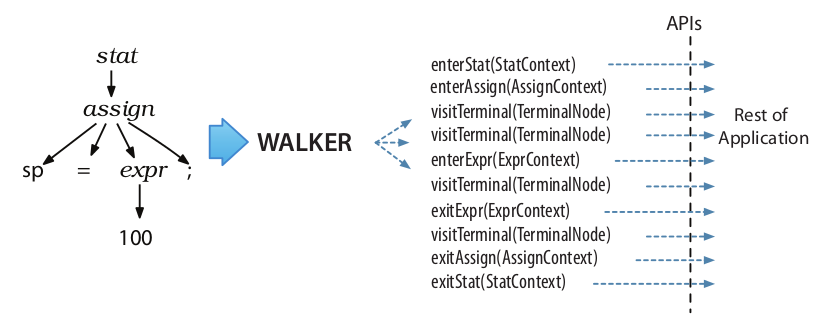
\includegraphics[width=0.8\textwidth]{images/antlrlistener.png}
  \caption{Sequence of calls made to the listener by ParseTreeWalker \cite{parr2013definitive}}
\end{figure}

The other mechanism is for ANTLR to generate a visitor interface from the grammar. This interface generates a visit method for each rule. The walker performs a depth-first walk of the tree and to initiate a walk of the tree, the application specific code would create a visitor implementation and call visit. The generate visitor interface contains default implementations for the visitor methods. This avoids having to override every method and focus on the methods of interest. \newline \par

\begin{figure}[H]
  \centering
  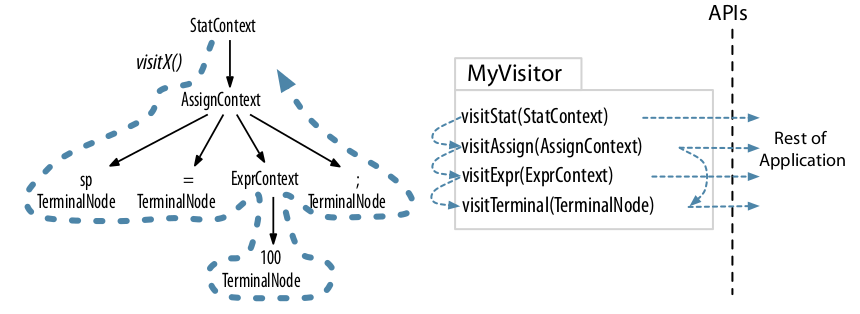
\includegraphics[width=0.8\textwidth]{images/antlrvisitors.png}
  \caption{Visitor pattern \cite{parr2013definitive}}
\end{figure}

The decided implementation of the tree-walking mechanism is the visitor interface. This implementation can be seen in dslWalkerVisitor. This mechanism was decided as it provides more control over the traversal of the tree. It allows the explicit call of the child nodes and retrieves the input values of the language based on the action node. This flexibility allows the walker to only have to visit the nodes which are needed. Visitor mechanisms also allow the function to return values. \newline \par

The Visitor mechanism allows for simple traversal of the tree, and acts as the interpreter for the system by executing application specific code based on each action and providing full control of the traversal. This differs from the Listener mechanism, which automatically visits every node and reacts to each node individually.

\section{Tweepy}

The second stage of implementation was to implement a way to interact with the Twitter API. The original design of the program to interact with the Twitter API was to build and create a RESTful web service. This original design idea was incredibly intricate and would have had to deal with low-level functionality including HTTP requests, authentication and rate limits and this implementation would be very time consuming, prone to error and outside the scope of the project. The Tweepy API is a convenient way to access the Twitter API with Python, as it includes a set of classes and methods that represent Twitter's models and API endpoints. Tweepy handles implementation details such as:
\begin{itemize}
    \item Data encoding and decoding
    \item HTTP requests
    \item Results pagination
    \item OAuth authentication
    \item Rate limits
    \item Streams
\end{itemize}
Tweepy provides a simple way to deal and interact with the Twitter API and provided all of the functionality of the Twitter API. This allows more resources to be focused on the main scope of the project, to design, implement and focus on the functionality of the domain specific language without much concern as to how to interact with the Twitter API. \newline \par

The initial implementation of the Tweepy API is in execute file. Tweepy supports OAuth 1a (application-user), which is required to interact with the Twitter API. 'execute' provides a function 'tweepy\_auth()' which uses the consumer keys to generate a OAuthHandler, which is used to authenticate and access a Tweepy API object. \newline \par

The Tweepy API object is then passed to the DSLVisitorWalker, which is used to execute application specific code. Based on each action, the relevant input information is retrieved and stored in kwargs. Since the grammar of the domain specific language is closely aligned with the Twitter API, the key value pairs in kwargs are the parameter name and the parameter value. This allows for the Visitor method to dynamically get all the required and optional parameters and pass kwargs to the correct Tweepy API call based on the action. This method of implementation provides a much simpler way to interact with the Twitter API than building a RESTful service. As Tweepy is a Python library, it provides a lot more functionality than interacting directly with the native Twitter API. Tweepy provides different objects such as Status objects and User objects and provides a Twitter Stream which retrieves tweets in real time. The combination of these objects, StreamListeners and native Python allows for a much wider range of possibilities for automation than the native Twitter API. This functionality is implemented is `dsl-twitter-bots', which uses the Tweepy API to perform three different automation tasks. The first tasks `replyMentions' takes keywords and a loop-time to respond to mentions for $x$ amount of time based on the keywords. The function `execute' iterates until the sum of initiated date time and loop-time is greater than or equal to the current date time and retrieves the mentions every 30 seconds. The function retrieves only new mentions from the the initiated date time and will provide a customised response to the mentions with content which include the keywords. This implementation is simple using the Tweepy library. It provides the functionality to get the most recent mentions, iterate over each tweet in the mention, retrieve the contents of the tweet and respond based on a conditional statement. The other two bot scripts, followFollowers and favRetweetListener operate in a similar way. followFollowers retrieves a list of all the users followers, iterates over the list and checks if the user account follows the follower and then follows the follower if they do not. favRetweetListener uses a StreamListener to retrieve tweets in real time. The StreamLister is filtered by certain keywords and certain actions can be performed based on the tweets it retrieves. In this bot script, it checks if the tweet does not belong to the users account and if the tweet is not already tweeted or favourites then it performs these actions. Utilising the Tweepy API allows for a simple solution to implementing bot scripts. An alternative would have been to have this functionality built into the domain specific language with program constructs such as looping and recursion however this would have added complexity to the language which does not satisfy the needs of a novice user.

\section{Django}

Django is a Python-based free and open-source web framework that follows the model-view-template (MVT) architectural pattern. The model-view-template is a slightly different version to the traditional model-view-controller architecture, as Django controls the interactions between the Model and the View, resulting in a template. The template is a HTML file mixed with Django Template Language. \newline \par

The execution of the domain specific language and interacting with the Tweepy API does not require Django. Django acts as a container for the domain specific language, providing a simple and intuitive way to interact with the domain specific language. The interaction between Django and the domain specific language is through Djangos custom management commands. Django comes with a variety of command line utilities that can be invoked and provides the functionality for custom commands. Custom management commands provides an simple way to interact with the application via command line. \newline \par

The custom management command used to interact with the domain specific language is execute\_dsl, which takes two arguments, account\_id and campaign\_id. Django automatically produces an id field for every Model and these are the arguments to be passed to the management command. The Models can be created through the Django admin site. This is an automatic admin interface, which reads metadata from the models to provide a quick, model-centric interface where trusted users can manage content the site. The use of the Django management site is a temporary solution until the web application interface is implemented, which will provide the tools for a user to upload and execute the domain specific language. After the management command has been executed, it interacts with execute.py, which takes a TwitterAccount and TwitterCampaign as parameters. The file execute.py retrieves the API credentials, authorises the Tweepy object and provides the core functionality of interacting directly with the domain specific language as it builds the parser, parses the input and initiates the tree traversal. \newline \par

Using Django provides a simple solution for storing information about the Twitter Account and Twitter Campaigns and executing the domain specific language. Django also provides a testing-suite which uses the standard Python unittest module. The testing suite in Django provides a simple solution for writing and executing unit tests to test the complex and intricate aspects on the domain specific language. \newline \par